\documentclass[8pt]{beamer}

\usepackage[utf8]{inputenc}
\usepackage{default}
\usepackage{hyperref}
\usepackage{textpos}
\usetheme{Copenhagen}

\title{Deep Learning}
\subtitle{Learning High-degree Non-linear Models: \\
Enabling factors, tips and tricks}
\author{Tero Keski-Valkama}
\institute{
\includegraphics[height=1.4cm]{CybercomG_logo_Classic_RGB.png}}
\date{2016-08-24}

\addtobeamertemplate{frametitle}{}{%
\begin{textblock*}{100mm}(10.95cm,-0.8cm)

\includegraphics[height=0.8cm]{cybercom-blue.png}
\end{textblock*}}


\begin{document}

\frame{\titlepage}
 
\begin{frame}
\frametitle{A quick recap}
\begin{itemize}
 \item Deep learning refers to deep neural networks. It took about 10 years for neural network technology to
       surpass the issues they stalled with in the 1990s. In 00s, if an academic paper mentioned neural networks, it was less likely to be published than if not.
 \item 1990s networks were shallow, and hence relatively useless: It requires a bunch of non-trivial tricks to make deeper networks possible.
       This presentation will present the most important of these tricks.
 \item Neural networks are just complex non-linear models with lots of parameters. They are formed by layers of neurons, successive operations
       with an a linear combination of inputs from the previous layer and an activation function.
 \item In general, you always need a training set, a test set and a validation set. Typically you would divide your data into three parts,
       train the system with the training set, test if the system overfits with the test set, and finally for the final system you can validate
       that your metaparameters didn't just learn the test set using the validation set.
 \item Underfitting = high bias, overfitting = high variance
\end{itemize}

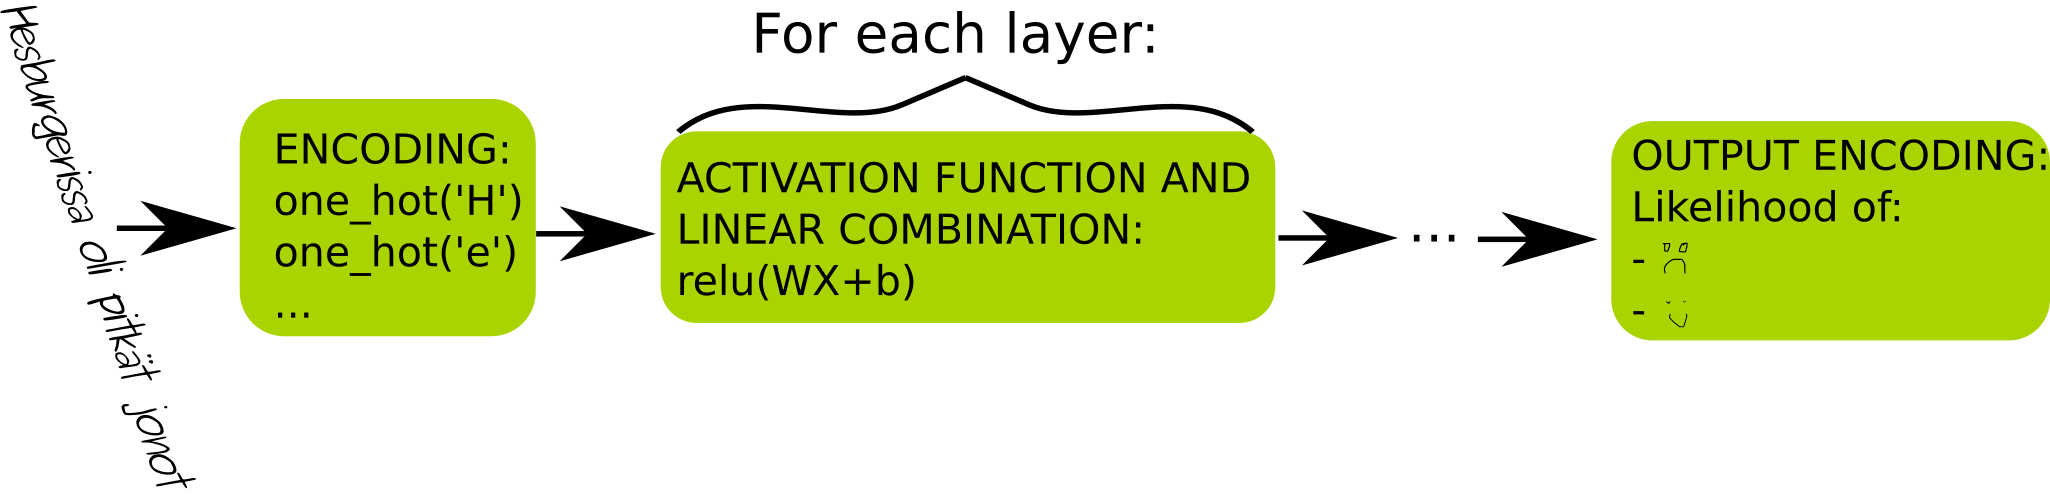
\includegraphics[width=0.9\textwidth]{./sentiment_analysis.png}

\end{frame}

\begin{frame}
\frametitle{Training Neural Networks 1/2}
\begin{itemize}
 \item Networks can be trained in a supervised fashion, with target outputs(labels), using backpropagation of error.
       The output error is known, and it is propagated backwards, layer by layer, estimating an error for each weight parameter.
       The weights are then updated using this error multiplied by the learning factor ($ << 1 $). Lots of learning steps makes
       the network learn the target function ($ input \rightarrow target\_output $)
 \item Non-linearities (activation functions) between the layers make the model interesting, compared to other statistical models.
 \item When the layers are getting smaller than the previous layer, the information is being compressed (or filtered), and the layer
 activations represent a higher abstraction level, a higher semantic level information about the signal.
\end{itemize}
\end{frame}

\begin{frame}
\frametitle{Training Neural Networks 2/2}
\begin{itemize}
 \item Unsupervised learning (no target output) can be done using backpropagation and autoassociativity ($ input \rightarrow input $),
 (or prediction: $ delayed\_input \rightarrow input $), or using Deep Belief Nets and Contrastive Divergence
 \footnote{\href{http://deeplearning.cs.cmu.edu/notes/yuxiong\_CD.pdf}{http://deeplearning.cs.cmu.edu/notes/yuxiong\_CD.pdf}}
 (minimizes the energy
 for generating real data-related distributions while maximizing the energy for "confabulations") for pairs of subsequent layers one by one.
 \item Metaoptimizing the learning hyperparameters and neural network structure should always be performed.
 \item A good platform to use for neural network experimentation is Google's TensorFlow, based on Python.
\end{itemize}

\centering{
\begin{tabular}{| c | c |}
\hline
Supervised & Unsupervised \\
Backpropagation & Contrastive Divergence \\
Non-energy-based Methods & Energy-based Methods \\
\hline
 
\end{tabular}}

\end{frame}

\begin{frame}
\frametitle{Tips \& Tricks}
 \begin{block}{Problems}
  \begin{itemize}
   \item Overlearning
   \item Getting stuck in local minima
   \item Exploding/diminishing gradients
  \end{itemize}
 \end{block}

 \begin{block}{Solutions}
  \begin{enumerate}
   \item Weight-sharing – less parameters
   \item Unsupervised pre-training – lots of data
   \item Near-linear activation functions
   \item Drop-out
   \item Gradient clipping
   \item Metaoptimization
   \item Bonus: Reservoir computing 
  \end{enumerate}
 \end{block}

\end{frame}

\begin{frame}
\frametitle{Regularization and Weight Sharing}
 \begin{itemize}
  \item Reducing the number of parameters or degrees of freedom of the model is regularization. Regularization prevents overfitting.
  \item In Convolutional Neural Networks, the weights are identical for each window, and window outputs are max-pooled (sub-sampling) to the next layer.
        This exploits the translational symmetry of the domain, and is often used for images.
  \item Regularization can also be done by introducing a loss term for weights, L2 norm is often used.
  \item As always in multiobjective optimization, the factors and slopes of the loss function components are important.
 \end{itemize}
 \begin{displaymath}
  RegularizedLoss = Loss + \alpha \cdot SquaredWeights^\beta
 \end{displaymath}
 \centering{
 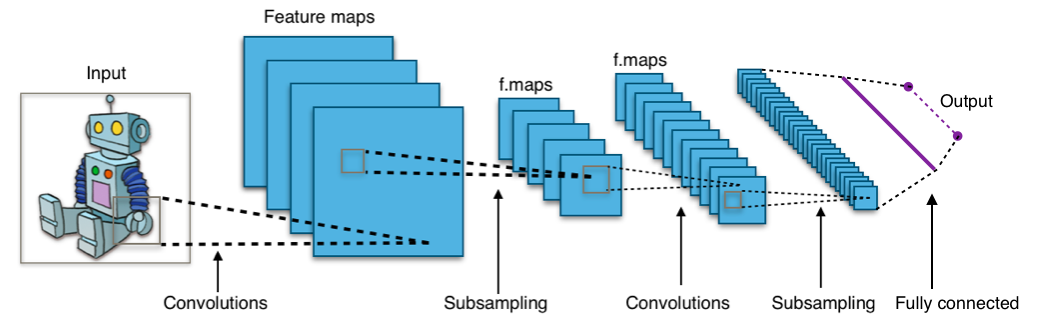
\includegraphics[width=0.9\textwidth]{./Typical_cnn.png}
 }
 \footnote{Image from: Aphex34, Wikipedia}
\end{frame}

\begin{frame}
\frametitle{Unsupervised pre-training}
 \begin{itemize}
  \item Unsupervised pre-training makes use of a lot of unlabeled data, learning the overall structure of the domain,
        which can be fine-tuned with backpropagation for specific labels at a later stage. More data, less labels.
        \footnote{\href{http://www.jmlr.org/papers/volume11/erhan10a/erhan10a.pdf}{http://www.jmlr.org/papers/volume11/erhan10a/erhan10a.pdf}}
  \item This could be thought of as "pre-training as regularization", or approaching neural reinforcement learning.
  \item Free pre-trained models are available from Google and Oxford University. Mostly convolutional nets trained on images and video.
        \footnote{\href{http://www.vlfeat.org/matconvnet/pretrained/}{http://www.vlfeat.org/matconvnet/pretrained/}}
  \item The models are taught using for example greedy DBN Contrastive Divergence or other autoencoding methods.
  \item In general, neural networks get better when trained on a different task with similar data.
        \footnote{\href{http://blogs.microsoft.com/next/2015/12/10/microsoft-researchers-win-imagenet-computer-vision-challenge/}
        {http://blogs.microsoft.com/next/2015/12/10/microsoft- \\ researchers-win-imagenet-computer-vision-challenge/}}
 \end{itemize}
\end{frame}

\begin{frame}
\frametitle{Near-linear Activation Functions}
 \begin{itemize}
  \item Deep neural networks are effective because of non-linear activation functions – Stacking linear
        layers only reduces to a single linear layer.
  \item However, non-linearities are challenging to learn. Minimizing the non-linearity has been shown to
        be really useful. Deep neural networks can be trained without unsupervised pre-training if rectifier
        activation functions are used. (otherwise cannot)
 \end{itemize}
\begin{columns}
\begin{column}{0.5\textwidth}
 \begin{figure}[h]
   \caption{Rectifier}
   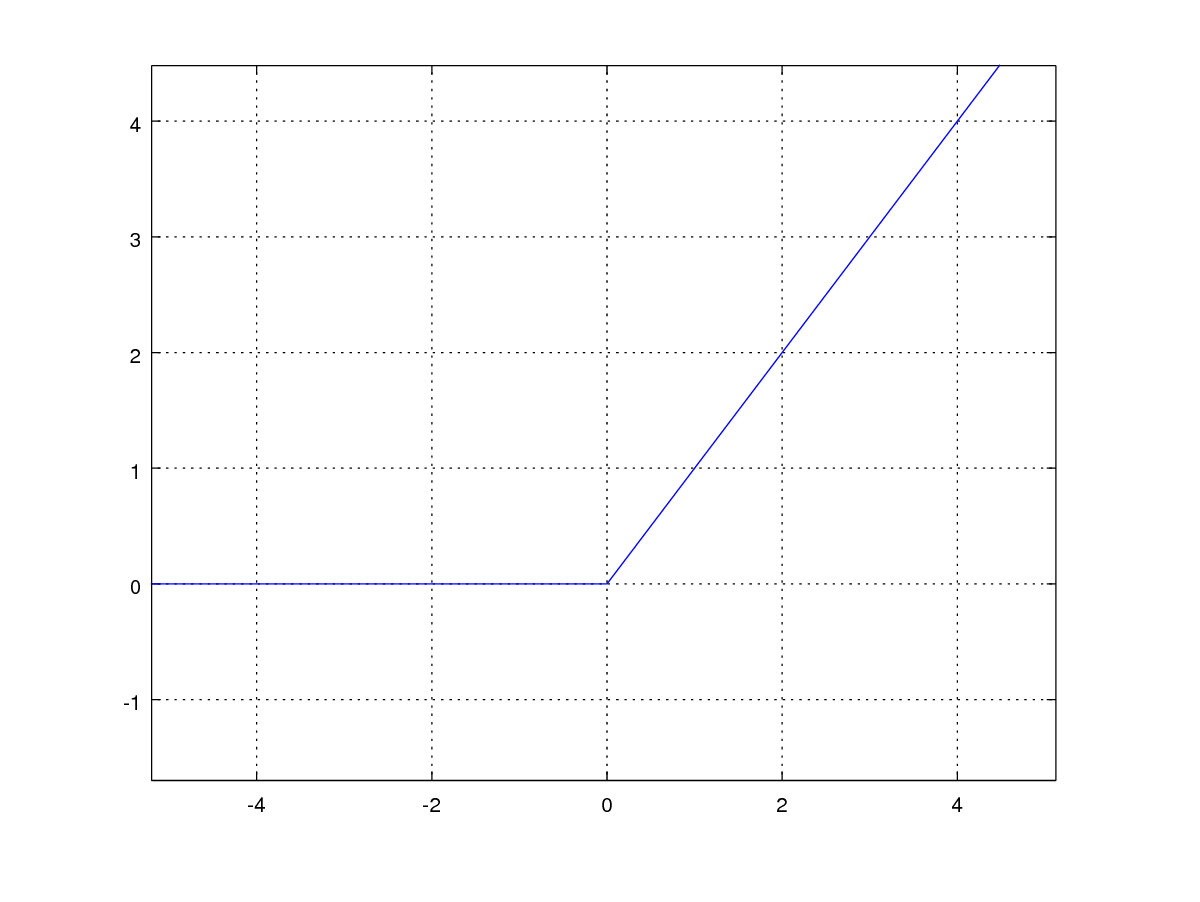
\includegraphics[width=0.9\textwidth]{./rect.png}
 \end{figure}
\end{column}
\begin{column}{0.5\textwidth}
 \begin{figure}[h]
   \caption{Leaky Rectifier}
   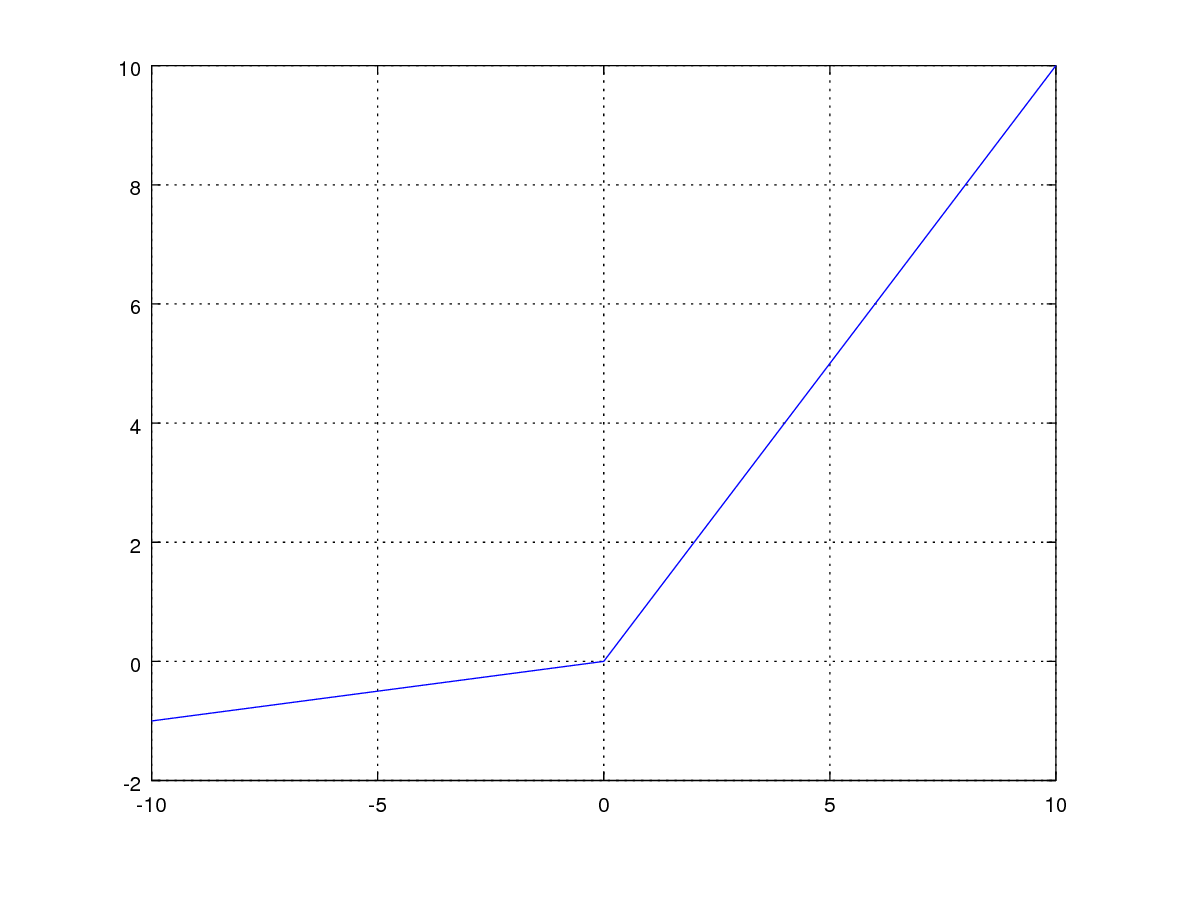
\includegraphics[width=0.9\textwidth]{./leaky_rect.png}
 \end{figure}
\end{column}
\end{columns}
\end{frame}

\begin{frame}
\frametitle{Drop-out}
 \begin{itemize}
  \item Dropout is a very effective strategy for preventing overfitting.
        \footnote{\href{https://www.cs.toronto.edu/~hinton/absps/JMLRdropout.pdf}{https://www.cs.toronto.edu/~hinton/absps/JMLRdropout.pdf}}
  \item In practice it means randomly dropping out for example half of the internal representation neurons and their output weights for each
        training step, and scaling the outputs accordingly.
  \item Learning is done by the randomly thinned networks, and the final use is done using the whole network.
  \item This prevents neurons from co-adapting with each other, and learn features more independently. I.e. one neuron learns one feature,
        not multiple neurons learning one feature.
  \item It is a very strong method against overfitting, and should be almost always used.
  \item Analogous to Random Forests or Ensemble Averaging Committee Machine.
  \item The expense is more learning iterations.
 \end{itemize}
 \centering{
   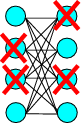
\includegraphics[width=0.1\textwidth]{./dropout.png}
 }
\end{frame}

\begin{frame}
\frametitle{Gradient clipping}
 \begin{itemize}
  \item Gradient explosion happens in backpropagation when the squared error gradients are amplified through activation functions
        of multiple layers. This typically causes infinities and divergence. Limited activation functions (sigmoid, tanh) are prone to this behavior.
  \item Gradients are often clipped to some maximum absolute value to prevent infinities.
  \item Gradients can also diminish to zero, when a small change in internal representation means a too large change in output. If
        a gradient goes to zero, it means it continues to be zero in backpropagation towards input. Adding noise might help the system in escaping local plateaus.
  \item Microsoft uses special one-bit gradients only signifying the direction of change, which is always non-zero.
        \footnote{\href{https://www.microsoft.com/en-us/research/publication/1-bit-stochastic-gradient-descent-and-application-to-data-parallel-distributed-training-of-speech-dnns/}
        {https://www.microsoft.com/en-us/research/publication/1-bit-stochastic-gradient-descent-and-application-to-data-parallel-distributed-training-of-speech-dnns/}}

 \end{itemize}
 \centering{
   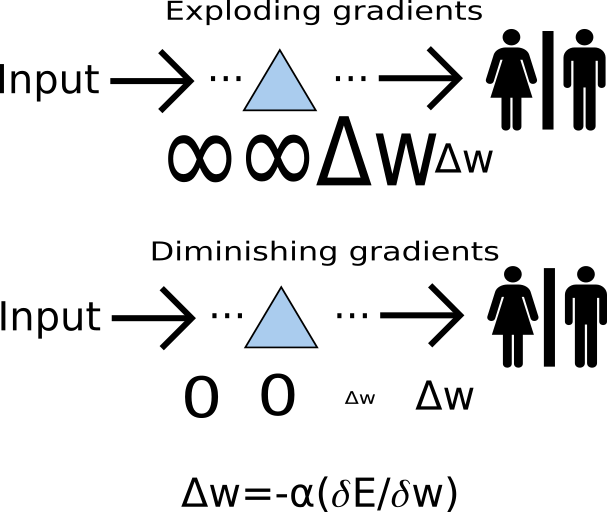
\includegraphics[width=0.3\textwidth]{./gradients.png}
 }
\end{frame}

\begin{frame}
\frametitle{Metaoptimization / Hyperparameter Tuning}
 \begin{itemize}
 \item With increased computational capacity we have better capability for metaoptimization.
 \item Metaoptimization means finding optimal network structures and learning parameters by running the learning multiple times with varying parameters.
 \item Two variants: Automatic Bayesian optimization and graphical optimization.
 \item Automatic Bayesian optimization should be used for stand-alone purposes, it finds good parameters without human aid.
       Parameter values to test are picked automatically.
 \item Graphical optimization is often better when human is available, and it also helps in understanding the system. You should sample
       parameter values randomly, instead of using an uniform grid.
 \item Process:
\begin{enumerate}
 \item Pick random values for 1-2 parameters
 \item Run the training for a while (i.e. 1 hour)
 \item Save the latest test set loss (not the best one)
 \item Draw a graph
\end{enumerate}
 \item Note that sometimes random noise causes apparent optimums. Always note that the other measured points are in agreement.
 \end{itemize}
 \centering{
   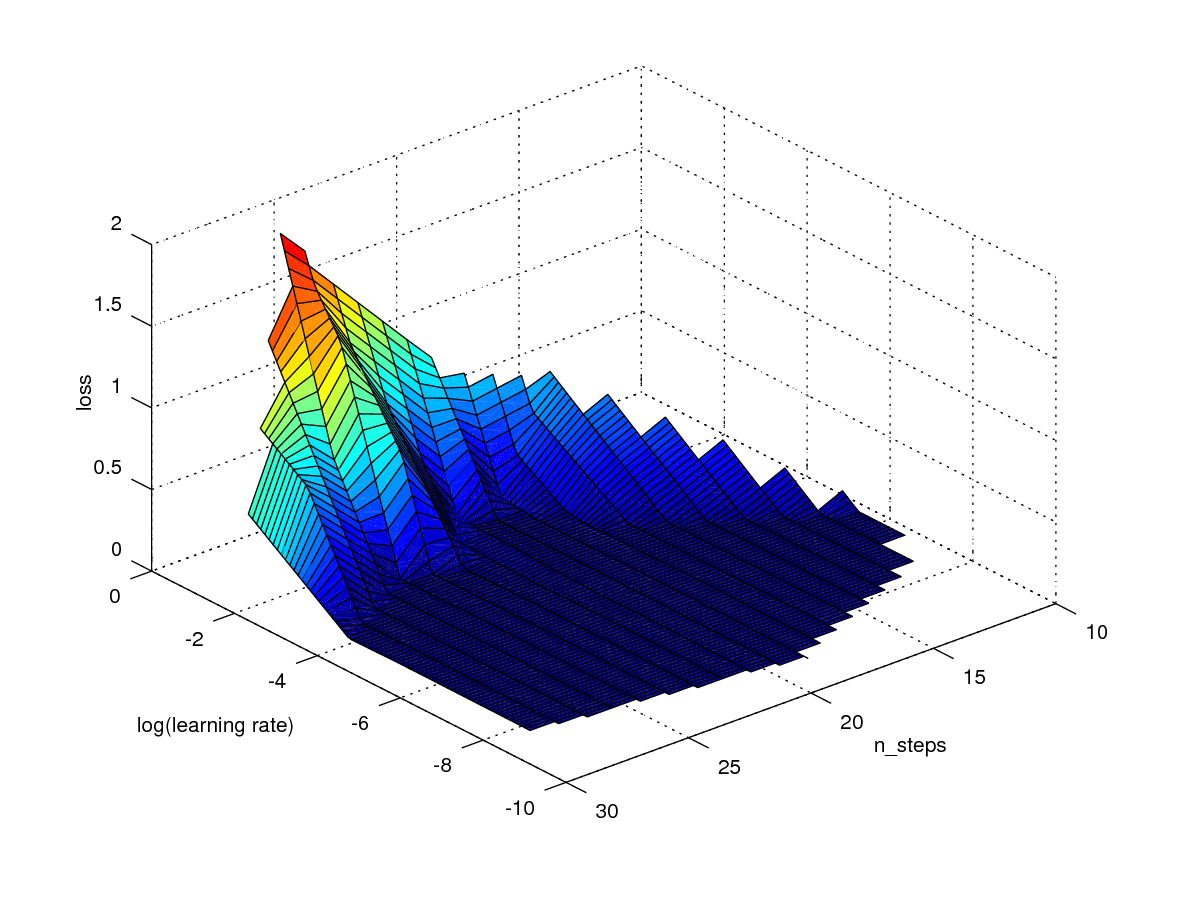
\includegraphics[width=0.3\textwidth]{./lr1_isom.png}
 }
\end{frame}

\begin{frame}
\frametitle{Metaoptimization / Hyperparameter Tuning}
 \centering{
   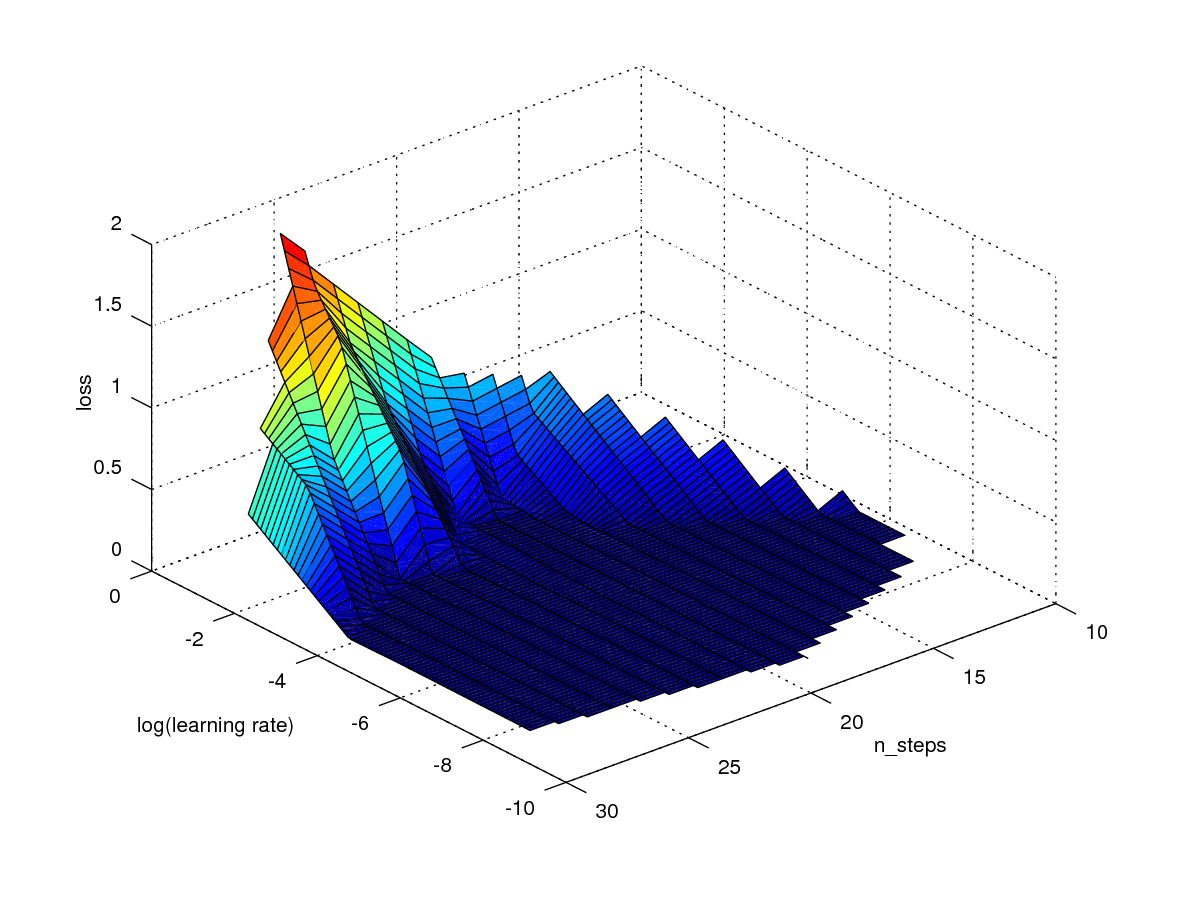
\includegraphics[width=\textwidth]{./lr1_isom.png}
 }
\end{frame}

\begin{frame}
\frametitle{Reservoir computing}
 \begin{itemize}
 \item A common name for methods that utilize a large, pre-initialized network, and then train a simple linear model with this large reservoir.
 \item Based on the observation that neural networks tend to learn mostly on the final layers anyhow.
 \item For example: Echo-State Networks
       \footnote{\href{http://minds.jacobs-university.de/sites/default/files/uploads/papers/PracticalESN.pdf}
                      {http://minds.jacobs-university.de/sites/default/files/uploads/\\papers/PracticalESN.pdf}}
       , Extreme Learning Machine
       \footnote{\href{https://www.researchgate.net/profile/Chee\_Siew/publication/4116697\_Extreme\_learning\_machine\_A\_new\_learning\_scheme\_of\_feedforward\_neural\_networks/links/00b4952f8672c66db1000000.pdf}
                      {https://www.researchgate.net/profile/Chee\_Siew/publication/\\4116697\_Extreme\_learning\_machine\_A\_new\_learning\_scheme\_of\_feedforward\\\_neural\_networks/links/00b4952f8672c66db1000000.pdf}}
       .
 \item Fast to train, work very well in domains where semantic depth is not required.
 \item Each neuron in the recurrent echo-state network reservoir represents a single non-linear signal response. The echo-state network learns an arbitrary response by
       fitting a linear combination of these responses to the desired output signal. Analogous to Fourier decomposition where any linear response
       can be decomposed in frequency plane, as a weighted sum of discrete cosine responses.
 \item Adding noise to the activation function arguments is critical for echo-state networks.
 \item Extreme Learning Machine fits a linear combination of a large reservoir of non-linear responses in a similar way but for feed-forward networks.
       Activation functions used in the ELM network used can be any mixture of infinitely differentiable functions, e.g. sigmoid, radial basis, sine, cosine,
       exponential, and many nonregular functions.
\end{itemize}
\end{frame}

\begin{frame}
\frametitle{What did we learn?}
 \begin{itemize}
  \item To make deep neural networks actually do anything useful, you need a bag of tricks:
  \item Regularization: Managing the number of parameters
  \item Pre-training with massive datasets
  \item Rectifier activation functions
  \item Dropout
  \item Gradient clipping
  \item These should be always used where relevant. In addition, the network structure and learning parameters should always be meta-optimized.
  \item Further reading, for example:
        \footnote{\href{https://www.linkedin.com/pulse/what-i-learned-from-deep-learning-summer-school-2016-hamid-palangi}
        {https://www.linkedin.com/pulse/what-i-learned-from-deep-\\learning-summer-school-2016-hamid-palangi}}
  \item The next lectures will be about:
  \begin{itemize}
    \item Data encoding / representation
    \item TensorFlow and meta-optimization
  \end{itemize}
 \end{itemize}
\end{frame}

\end{document}

